\documentclass{llncs}
\usepackage{graphicx,pgfplotstable}

\begin{document}

%
% ---- Title page
%
	
\title{Performance modelling and simulation of skewed demand in complex systems}
\subtitle{Interim Report}

\author{Stephen Shephard SN: 160337206}

\institute{School of Computing Science, Newcastle University, Newcastle upon Tyne, NE1 7RU\\
	\email{s.shephard2@newcastle.ac.uk}}

\maketitle

\vspace*{\fill}
\begin{center}

\includegraphics[width=\textwidth]{img/ncllogo}
\end{center}
\newpage

%
% ---- Introduction
% ---- A short introduction to the project (this should set the scene for the project and motivate why the project is interesting). 
%

\section{Introduction}

There are many high-profile examples of whole IT systems brought down by skewed customer demand for part of their services.  Customers were prevented from using any part of the London 2012 Olympic ticketing website on launch day to avoid demand overloading the system \cite{RN1067}.  HBO Go was brought down by demand for the finale of ``True Detective'' \cite{RN1066}.  Apple's iTunes Store suffered outage on the launch day of the iPhone 7 (new iPhone registration is carried out via an iTunes function) \cite{RN1068}.

It is possible to design and build more resilient systems through effective use of Cloud technologies where higher than normal demand for one function or type of resource would not block access to the others.  Skewed demand may be isolated so that it only affects parts of a system, or shared equally between different components. (The system may also adapt to demand by elastic scaling of resources, but this will be beyond the scope of the project).

In a complex system we need to examine how these components interact.  What impact would a particular choice of middleware have on the demand at the database, for example?  To examine these questions we will choose an approach to build models of selected Cloud technology components that may be combined into different system architectures.

%
% ---- A clear statement of the high-level aim of the project and a list of the scientific objectives of the work. 
%

\section{Aims and Objectives}

The aim is to demonstrate that PEPA (Performance Evaluation Process Algebra) \cite{RN1051} may be used to construct models that are good predictors of the behaviour of real systems under skewed demand scenarios, and provide insights into the effectiveness of Cloud technologies for handling skewed demand.

\subsection{Objectives}
\begin{enumerate}
	\item Show that distributed databases and middleware queues may be modelled in PEPA
	\item Show that these PEPA component models may be used to test skewed demand 
	\item Show that the component models may be composed into system models and their behaviour under test is different to the components alone
	\item Build test system architectures for the PEPA models and show that the test system behaviour matches that predicted by the models
	\item Identify areas of further work
\end{enumerate}

\section{Method}

We will consider an example system based on the Olympic ticketing use case above, where tickets will be available for a number of sports.  Such an application may be generalised to any system for allocating and releasing other resources with variable demand.

In all system architectures users will access the system from a web-based front end.  Tickets will be stored in a database partitioned across several data stores.  In between the web servers and database will be worker applications to service user requests, connected to the web servers by some middleware (see Figure \ref{figure:architecture}).

\begin{figure}
	\caption{Ticketing application distributed architecture}
	\label{figure:architecture}
	\centering
	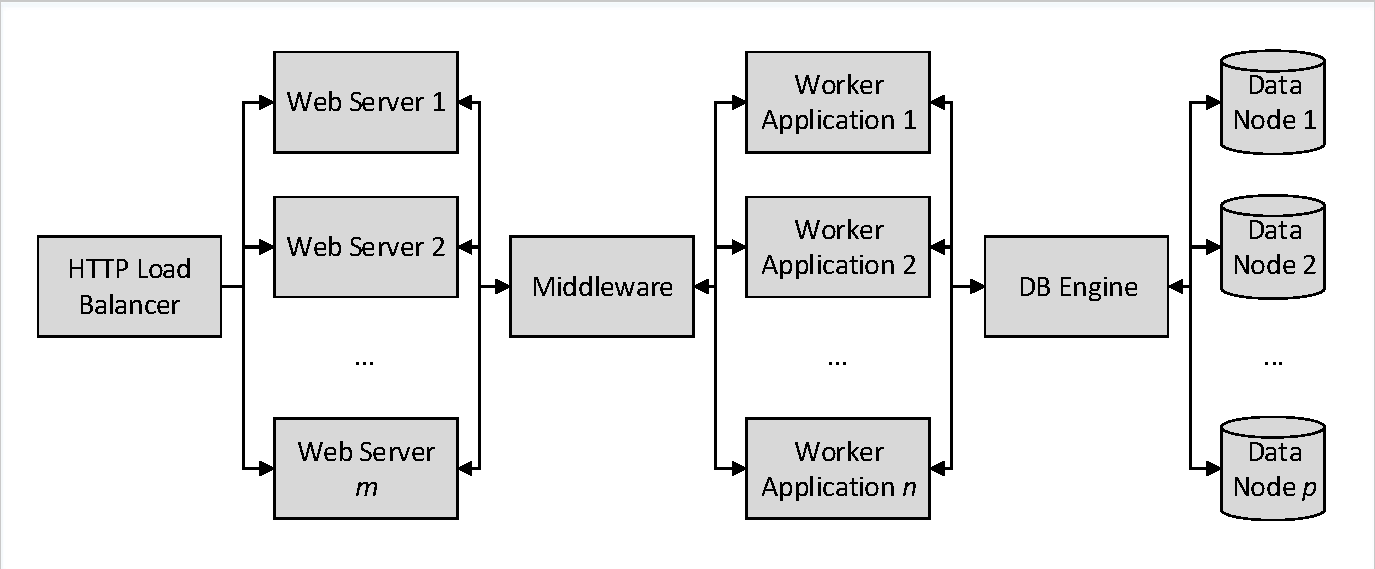
\includegraphics[trim = 5 5 5 5, clip, width=\textwidth]{img/application}
\end{figure}

The components modelled will be distributed database nodes using horizontal partitioning \cite{RN68}, distributed database nodes with Cassandra-style replication \cite{RN1050} and a shared middleware queue \cite{RN65}.  These will be tested then composed into three system architectures - \textit{simple microservices} (separate worker applications and databases for Athletics and Cycling tickets), \textit{distributed database via a shared queue}  and \textit{distributed database with replication via a shared queue}.  Finally these system architectures will be built on Microsoft Azure and compared with the models.

%
% ---- A brief description of the progress so far made (i.e. areas researched, analysis undertaken, software or model development undertaken). 
%

\section{Progress to date}

I've completed the following tasks to date. See Table \ref{table:plan} for done dates and percentage completion against each of the tasks in the timed work plan.
\begin{itemize}
	\item Reviewed ``Investigating Cloud Technologies to Maximise Availability of Oversubscribed Resources'' for Research Skills module
	\item Agreed initial scope of ``Performance modelling and simulation of skewed demand in complex systems'' and submitted Ethics form
	\item Carried out further background learning and research into technology choices
	\item Set up GitHub structure for Model, Code and Report development and produced outline and timed work plans
	\item Produced and tested PEPA component models
	\item Produced PEPA system models
\end{itemize}

%
% ---- A timed work plan for completion of the project.
%

\section{Timed work plan}

There is a detailed Microsoft Project Plan in the project git repository at \url{https://github.com/sshephard2/msc-project}.  Table \ref{table:plan} shows a high-level summary.

\subsection{Risks}
\begin{enumerate}
	\item Development may take longer than expected due to lack of experience in Java Spring or AngularJS.  In mitigation, I have already developed a simple Angular to Cassandra Java Spring application during the Learning phase.
	\item The models may not after all be good matches to the behaviour of real systems.  There is contingency time in the plan, but this may also be an interesting result for discussion.
\end{enumerate}

\begin{table}[h!]
	\begin{center}
		\caption{Planned tasks (subtasks in italics)}
		\label{table:plan}
		\pgfplotstabletypeset[
		col sep=comma,
		string type,
		columns/Task/.style={column name=Task, column type={p{.45\textwidth}}},
		columns/Start/.style={column name=Start, column type={p{.2\textwidth}}},
		columns/End/.style={column name=End, column type={p{.2\textwidth}}},
		columns/Complete/.style={column name=Complete, column type={p{.1\textwidth}}},
		every head row/.style={before row=\hline,after row=\hline},
		every last row/.style={after row=\hline},
		]{data/plan.csv}
	\end{center}
\end{table}


%
% ---- Bibliography ----
%

\newpage

\bibliographystyle{splncs03}
\bibliography{references}

\end{document}